
% This LaTeX was auto-generated from MATLAB code.
% To make changes, update the MATLAB code and republish this document.

\documentclass{article}
\usepackage{graphicx}
\usepackage{color}

\sloppy
\definecolor{lightgray}{gray}{0.5}
\setlength{\parindent}{0pt}

\begin{document}

    
    
\subsection*{Contents}

\begin{itemize}
\setlength{\itemsep}{-1ex}
   \item PROMBLEM 1-1:NUMERICAL BASIC
   \item PROBLEM 1-3:HORNER METHOD
   \item PROBLEM 2-1:LU DECOMPOSITION SOLVE A LINEAR EQUATION Ax=b
   \item PROBLEM 2-2:CHOLESKY DECOMPOSITION SOLVE LINEAR EQUATION Ax=b
   \item PROBLEM 2-4:QR DECOMPOSITION
   \item PROBLEM 2-7:SOLVE LINEAR EQUATION (GAUSS\_SEIDEL \&\& JACOBI)
   \item PROBLEM 3-2:SOLVE NONLINEAR EQUATION
   \item FUNCTION(A)
   \item FUNCTION(B)
   \item PLOT
   \item FIND ROOTS
   \item GET UNIQUE ROOT FROM THE LIST LIST-\ensuremath{>}SET
   \item PROBLEM 4-1 LAGRANGE INTERPLATION
   \item PROBLEM 4-2 HERMITE INTERPLATION
   \item PROBLEM 4-6 PROXIMATTION AND RUNGE PHOMENON
   \item PROBLEM 5-3 NUMERICAL INTEGRATION
   \item PROBLEM 6-1 SOLAVE DIFFERETIAL EQUATION
\end{itemize}


\subsection*{PROMBLEM 1-1:NUMERICAL BASIC}

\begin{par}
the value 'forward' is the first section of the problem the 'backword' is the second,meaning form the end to begin to get the numerical answer. 'exact' is the true answer of the series
\end{par} \vspace{1em}
\begin{par}
$$\frac{1}{2}\left(\frac{3}{2}-\frac{1}{n}-\frac{1}{n+1}\right)$$
\end{par} \vspace{1em}
\begin{par}
'term' is the term of the series $$\frac{1}{n^2-1}$\$ this section use function nnl\_serial1 to calculate,single function(nnl\_serial1.m)
\end{par} \vspace{1em}
\begin{verbatim}
term1_1=@(n)1/(n^2-1);
start=2;
for k=2:2:6
	forward(k)=nnl_serial1(term1_1,start,10^k,1);
	backward(k)=nnl_serial1(term1_1,10^k,start,-1);
	exact(k)=1/2*(3/2-1/10^k-1/(10^k+1));
end
disp("PROMBLEM 1-1:ANSWER:================================")
disp(["S_{10^2}:FOR / BACK",forward(2),backward(2),exact(2)]);
disp(["S_{10^4}:FOR / BACK",forward(4),backward(4),exact(4)]);
disp(["S_{10^6}:FOR / BACK",forward(6),backward(6),exact(6)]);
\end{verbatim}

        \color{lightgray} \begin{verbatim}PROMBLEM 1-1:ANSWER:================================
    "S_{10^2}:FOR / BACK"    "0.74005"    "0.74005"    "0.74005"

    "S_{10^4}:FOR / BACK"    "0.74985"    "0.7499"    "0.7499"

    "S_{10^6}:FOR / BACK"    "0.74985"    "0.75"    "0.75"

\end{verbatim} \color{black}
    

\subsection*{PROBLEM 1-3:HORNER METHOD}

\begin{par}
this program use hornercal(hornercal.m)
\end{par} \vspace{1em}
\begin{verbatim}
ans_1_3=hornercal(ones(1,50),1.00001);
disp(["ANSWER 1-3:========================================",ans_1_3]);
\end{verbatim}

        \color{lightgray} \begin{verbatim}    "ANSWER 1-3:========================================"    "51.0128"

\end{verbatim} \color{black}
    

\subsection*{PROBLEM 2-1:LU DECOMPOSITION SOLVE A LINEAR EQUATION Ax=b}

\begin{par}
LU decomposition $$A=LU$\$ A:'A\_mat\_2\_1' L:l\_2\_1 U;u\_2\_1 this section use lude(lude.m)
\end{par} \vspace{1em}
\begin{verbatim}
A_mat_2_1=[31,-13,0,0,0,-10,0,0,0;-13,35,-9,0,-11,0,0,0,0;0,-9,31,-10,...
    0,0,0,0,0;0,0,-10,79,-30,0,0,0,-9;0,0,0,-30,57,-7,0,-5,0;0,0,0,0,-7,...
    47,-30,0,0;0,0,0,0,0,-30,41,0,0;0,0,0,0,-5,0,0,27,-2;0,0,0,-9,0,0,0,...
    -2,29];
[l_2_1,u_2_1]=lude(A_mat_2_1);
disp("ANSWER 2-1:==============================================");
disp([l_2_1,u_2_1]);
\end{verbatim}

        \color{lightgray} \begin{verbatim}ANSWER 2-1:==============================================
  列 1 至 3

   1.000000000000000                   0                   0
  -0.419354838709677   1.000000000000000                   0
                   0  -0.304585152838428   1.000000000000000
                   0                   0  -0.353872899362565
                   0                   0                   0
                   0                   0                   0
                   0                   0                   0
                   0                   0                   0
                   0                   0                   0

  列 4 至 6

                   0                   0                   0
                   0                   0                   0
                   0                   0                   0
   1.000000000000000                   0                   0
  -0.397554925856813   1.000000000000000                   0
                   0  -0.156943635949482   1.000000000000000
                   0                   0  -0.653976718762685
                   0  -0.112102597106773  -0.017545375758242
  -0.119266477757044  -0.083390882105164  -0.014226814779801

  列 7 至 9

                   0                   0                   0
                   0                   0                   0
                   0                   0                   0
                   0                   0                   0
                   0                   0                   0
                   0                   0                   0
   1.000000000000000                   0                   0
  -0.024618525643365   1.000000000000000                   0
  -0.019962137562965  -0.092316470259097   1.000000000000000

  列 10 至 12

  31.000000000000000 -13.000000000000000                   0
                   0  29.548387096774192  -9.000000000000000
                   0                   0  28.258733624454148
                   0                   0                   0
                   0                   0                   0
                   0                   0                   0
                   0                   0                   0
                   0                   0                   0
                   0                   0                   0

  列 13 至 15

                   0                   0 -10.000000000000000
                   0 -11.000000000000000  -4.193548387096774
 -10.000000000000000  -3.350436681222708  -1.277292576419214
  75.461271006374346 -31.185628742514972  -0.451999227351748
                   0  44.601999677471376  -7.179694519317161
                   0                   0  45.873192637131794
                   0                   0                   0
                   0                   0                   0
                   0                   0                   0

  列 16 至 18

                   0                   0                   0
                   0                   0                   0
                   0                   0                   0
                   0                   0  -9.000000000000000
                   0  -5.000000000000000  -3.577994332711314
 -30.000000000000000  -0.784718179747412  -0.561543439982356
  21.380698437119459  -0.513187420344639  -0.367236336322372
                   0  26.413084921470535  -2.419995764952248
                   0                   0  27.389504332776948

\end{verbatim} \color{black}
    

\subsection*{PROBLEM 2-2:CHOLESKY DECOMPOSITION SOLVE LINEAR EQUATION Ax=b}

\begin{par}
cholesky decomposition solve Ax=b $$LL^Ty=b$\$ this section use nnl\_cholesky(nnl\_cholesky.m)
\end{par} \vspace{1em}
\begin{verbatim}
A_mat_2_2=[7,1,-5,1;1,9,2,7;-5,2,7,-1;1,7,-1,9];
b_vec_2_2=[13;-9;6;0];
l_mat_2_2=nnl_cholesky(A_mat_2_2);
y_2_2=b_vec_2_2\l_mat_2_2;
ans_2_2=transpose(y_2_2)\transpose(l_mat_2_2);
disp(["ANSWER 2-2:=======================================",ans_2_2])
\end{verbatim}

        \color{lightgray} \begin{verbatim}  列 1 至 2

    "ANSWER 2-2:======================================="    "14.0554"

  列 3 至 5

    "-15.1366"    "-5.49165"    "-15.1366"

\end{verbatim} \color{black}
    

\subsection*{PROBLEM 2-4:QR DECOMPOSITION}

\begin{par}
QR decomposition $$A=QR$\$ this section use nnl\_qr(nnl\_qr.m)
\end{par} \vspace{1em}
\begin{verbatim}
A_mat_2_4=[1 1 0 0;-1 3 -1/2 1/2;-2 2 3/2 1/2;-2 2 -1/2 5/2];
[q_mat_2_4,r_mat_2_4]=nnl_qr(A_mat_2_4);
disp(["ANSWER 2-4:========================================","Q:","R:"]);
disp(q_mat_2_4);
disp(r_mat_2_4)
\end{verbatim}

        \color{lightgray} \begin{verbatim}    "ANSWER 2-4:========================================"    "Q:"    "R:"

  列 1 至 3

   0.316227766016838  -0.316227766016838  -0.632455532033676
   0.707106781186548   0.707106781186547  -0.000000000000000
   0.258198889747161  -0.258198889747161   0.774596669241484
  -0.577350269189626   0.577350269189626   0.000000000000000

  列 4

  -0.632455532033676
   0.000000000000000
  -0.516397779494322
  -0.577350269189626

  列 1 至 3

   3.162277660168379  -3.162277660168379  -0.474341649025257
   0.000000000000000   2.828427124746190  -0.353553390593274
                   0                   0   1.549193338482967
  -0.000000000000000   0.000000000000001   0.000000000000001

  列 4

  -2.055480479109447
   0.353553390593274
  -1.032795558988644
  -1.154700538379252

\end{verbatim} \color{black}
    

\subsection*{PROBLEM 2-7:SOLVE LINEAR EQUATION (GAUSS\_SEIDEL \&\& JACOBI)}

\begin{verbatim}
f_A_2_7_cons=@(n,m_var,l_var,u_var)diag(repmat(m_var,[1,n]))+...
    diag(repmat(l_var,[1,n-1]),-1)+diag(repmat(u_var,[1,n-1]),1);

A_mat_2_7=arrayfun(f_A_2_7_cons,[10,20,30,50,100],repmat(3,[1,5]),...
    repmat(-1,[1,5]),repmat(-1,[1,5]),'UniformOutput',false);
b_mat_2_7=arrayfun(@f_b_2_7_cons,[10,20,30,50,100],repmat(2,[1,5]),...
    ones(1,5),'Uniformoutput',false);

solution_vec_2_7=cellfun(@nnl_jacobi_le,A_mat_2_7,b_mat_2_7,...
    {1e-5,1e-5,1e-5,1e-5,1e-5},'Uniformoutput',false);
disp("ANSWER 2-7:=========================================");
\end{verbatim}

        \color{lightgray} \begin{verbatim}ANSWER 2-7:=========================================
\end{verbatim} \color{black}
    

\subsection*{PROBLEM 3-2:SOLVE NONLINEAR EQUATION}



\subsection*{FUNCTION(A)}

\begin{verbatim}
f_3_2_a=@(x)x*cos(x)+2;

root_3_2_a=nnl_dfr(-4,4,f_3_2_a,1e-3);
disp(["ANSWER 3-2(a):========================================"]);
disp(root_3_2_a)
\end{verbatim}

        \color{lightgray} \begin{verbatim}    "THE WORST SITUATION ITER STEP:"    "13"    "SIMULATION NUMBER:"    "14"

ANSWER 3-2(a):========================================
   2.499023437500000

\end{verbatim} \color{black}
    

\subsection*{FUNCTION(B)}

\begin{verbatim}
var_0_num=100;

f_3_2_b=cell(1,var_0_num);
fd_3_2_b=cell(1,var_0_num);

for i=1:var_0_num
    f_3_2_b{i}=@(x)x^3+2*x^2+10*x-100;
    fd_3_2_b{i}=@(x)3*x^2+2*x+10;
end

var_0_3_2_b=linspace(-10,20,var_0_num);
tor_err=repmat(1e-4,[1,var_0_num]);

[root_3_2_root,root_3_2_step]=cellfun(@nnl_newton_nle,f_3_2_b,...
    fd_3_2_b,mat2cell(var_0_3_2_b,1,ones(1,var_0_num)),...
    mat2cell(tor_err,1,ones(1,var_0_num)),'Uniformoutput',false);

step_3_2=[];
for i=1:var_0_num
    step_3_2=[step_3_2,root_3_2_step{i}(1)];
end
scatter(var_0_3_2_b,step_3_2);
close

%%PROBLEM 3-6:FIND ROOT ON A SPECIAL SPAN AND PROSIMATE ERROR
f_3_6=@(x)hornercal([-4,16,35,-69,-102,45,54],x);
fd_3_6=@(x)hornercal([16,35*2,-69*3,-102*4,45*5,54*6],x);

x_3_6=linspace(-2,2,100);
y_3_6=arrayfun(f_3_6,x_3_6);
\end{verbatim}


\subsection*{PLOT}

\begin{verbatim}
plot(x_3_6,y_3_6);
\end{verbatim}


\subsection*{FIND ROOTS}

\begin{verbatim}
var_0_num=100;

cf_3_6=cell(1,var_0_num);
cfd_3_6=cell(1,var_0_num);

for i=1:var_0_num
    cf_3_6{i}=f_3_6;
    cfd_3_6{i}=fd_3_6;
end

var_0_3_6=linspace(-2,2,var_0_num);
tor_err=repmat(1e-4,[1,var_0_num]);

[root_3_6_root,root_3_6_step]=cellfun(@nnl_newton_nle,cf_3_6,cfd_3_6,...
    mat2cell(var_0_3_6,1,ones(1,var_0_num)),...
    mat2cell(tor_err,1,ones(1,var_0_num)),'Uniformoutput',false);
\end{verbatim}


\subsection*{GET UNIQUE ROOT FROM THE LIST LIST-\ensuremath{>}SET}

\begin{verbatim}
root_set=[];
for i=1:var_0_num
    root_set=[root_set,root_3_6_root{i}(1)];
end

root_set=uniquetol(root_set,1e-4);
\end{verbatim}

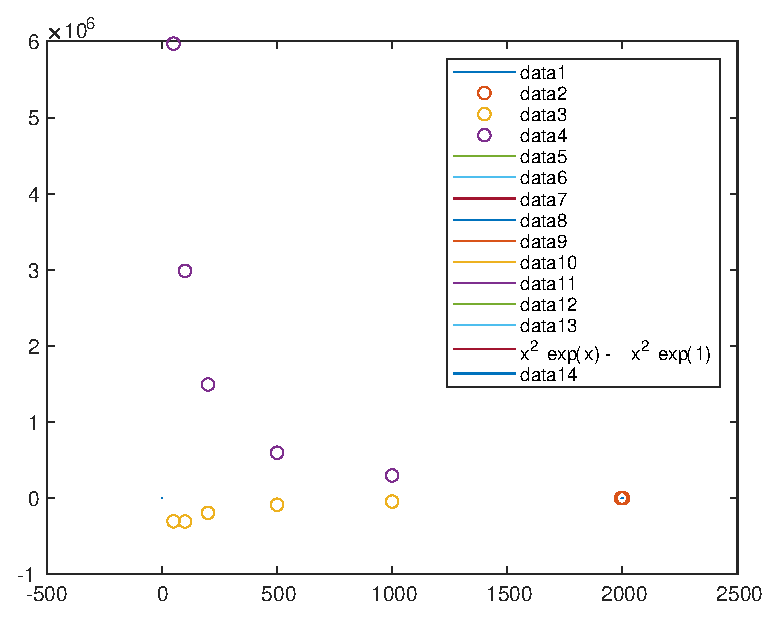
\includegraphics [width=4in]{main_01.eps}


\subsection*{PROBLEM 4-1 LAGRANGE INTERPLATION}

\begin{verbatim}
f_4_1=@(x)1/(1+x^2);
interval_4_1={2,1,1/2};
points_4_1=linspace(-5,5,100);
inter_4_1=cellfun(@nnl_lginter,{[-5,5],[-5,5],[-5,5]},{6,11,21},...
    {f_4_1,f_4_1,f_4_1},{points_4_1,points_4_1,points_4_1},...
    'Uniformoutput',false);
for i=1:length(interval_4_1)
    plot(points_4_1,inter_4_1{i});
    hold on;
end
\end{verbatim}

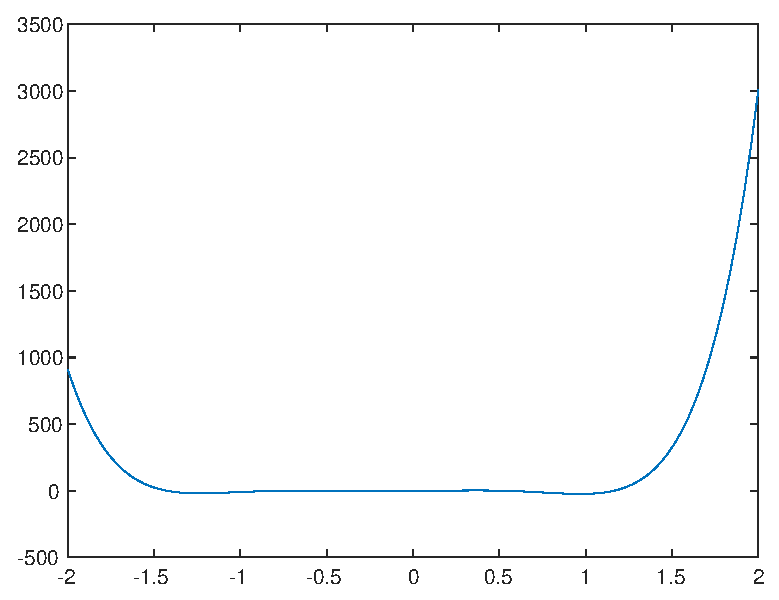
\includegraphics [width=4in]{main_02.eps}


\subsection*{PROBLEM 4-2 HERMITE INTERPLATION}

\begin{verbatim}
f_4_2_vec=@(x)1./(1+x.^2);
y_4_2=f_4_2_vec(points_4_1);
inter_4_2=cellfun(@spline,{points_4_1,points_4_1,points_4_1},...
    {y_4_2,y_4_2,y_4_2},'Uniformoutput',false);
for i=1:length(interval_4_1)
    plot(points_4_1,ppval(inter_4_2{i},points_4_1));
    hold on;
end
\end{verbatim}

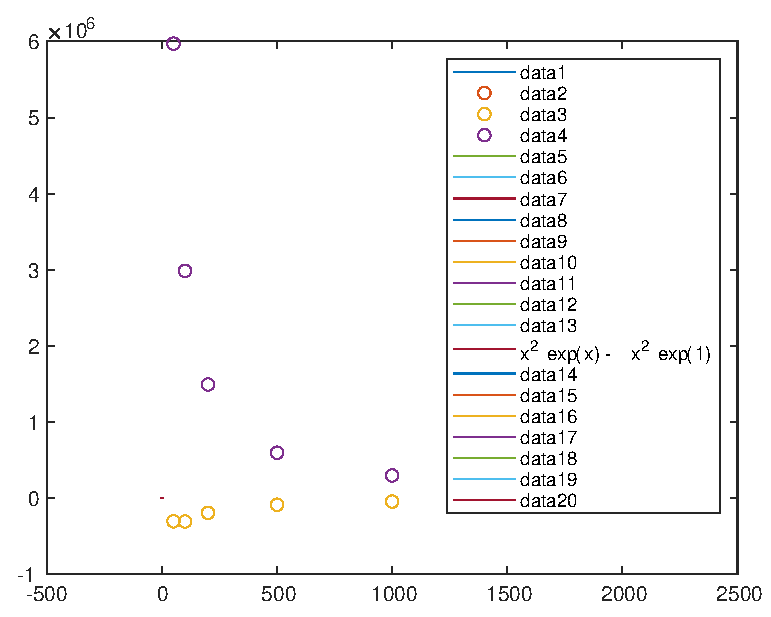
\includegraphics [width=4in]{main_03.eps}


\subsection*{PROBLEM 4-6 PROXIMATTION AND RUNGE PHOMENON}

\begin{verbatim}
y_4_6=nnl_lginter([1994,2003],10,[67.052,68.008,69.803,...
    72.024,73.400,72.063,74.669,74.487,74.065,76.777],...
    linspace(1994,2003,100))
close
plot(linspace(1994,2003,100),y_4_6);
hold on
scatter(linspace(1994,2003,10),[67.052,68.008,69.803,72.024,73.400,...
    72.063,74.669,74.487,74.065,76.777])
\end{verbatim}

        \color{lightgray} \begin{verbatim}
y_4_6 =

  列 1 至 3

  67.052000000000007  63.472134445073060  61.568918616356655

  列 4 至 6

  60.877136083466695  61.024007043830359  61.715640610832693

  列 7 至 9

  62.724935747349342  63.880822812041870  65.058742750553080

  列 10 至 12

  66.172265915613693  67.165757338522724  68.007999999999996

  列 13 至 15

  68.686692260680275  69.203740110588257  69.571269282990997

  列 16 至 18

  69.808286550827276  69.937923683564080  69.985201588899031

  列 19 至 21

  69.975256097078940  69.931970665826370  69.876964990946902

  列 22 至 24

  69.828892101601738  69.802999999999997  69.810917272878953

  列 25 至 27

  69.860625356606818  69.956583279050761  70.099973729517117

  列 28 至 30

  70.289042223075427  70.519503927433703  70.784995409247060

  列 31 至 33

  71.077551132273257  71.388087002219905  71.706875602346315

  列 34 至 36

  72.024000000000001  72.329775127216877  72.615127748285346

  列 37 至 39

  72.871927923838271  73.093266664527320  73.273676137650682

  列 40 至 42

  73.409290347316215  73.497945652749905  73.539221820230367

  列 43 至 45

  73.534425521882383  73.486519299123771  73.400000000000006

  列 46 至 48

  73.280731577909023  73.135737904348517  72.972961900289292

  列 49 至 51

  72.800997829592006  72.628804023567227  72.465403618284597

  列 52 至 54

  72.319581085601214  72.199582425107735  72.112826857229976

  列 55 至 57

  72.065637717655790  72.063000000000002  72.108351627231599

  列 58 至 60

  72.203415052845301  72.348075200054936  72.540309041446562

  列 61 至 63

  72.776171302518620  73.049839840388017  73.353723203646297

  列 64 至 66

  73.678631720868054  74.014012193702854  74.348244885683783

  列 67 至 69

  74.668999999999997  74.963649228416401  75.219726229287843

  列 70 至 72

  75.425428055269705  75.570147600806408  75.645025075789533

  列 73 至 75

  75.643504334979312  75.561877602795661  75.399799729960108

  列 76 至 78

  75.160750602194938  74.852421691756390  74.486999999999995

  列 79 至 81

  74.081319783428981  73.656849486816427  73.239478224938352

  列 82 至 84

  72.859062959256690  72.548694207585257  72.343634703247204

  列 85 至 87

  72.279881885594790  72.392301455988502  72.712275472353667

  列 88 至 90

  73.264804581361020  74.064999999999998  75.113896757949973

  列 91 至 93

  76.393515498551494  77.861095809496945  79.442419614545059

  列 94 至 96

  81.024138604452489  82.445015019236195  83.485980314589582

  列 97 至 99

  83.858911352669054  83.194018752051377  81.025736912694057

  列 100

  76.777000000000001

\end{verbatim} \color{black}
    
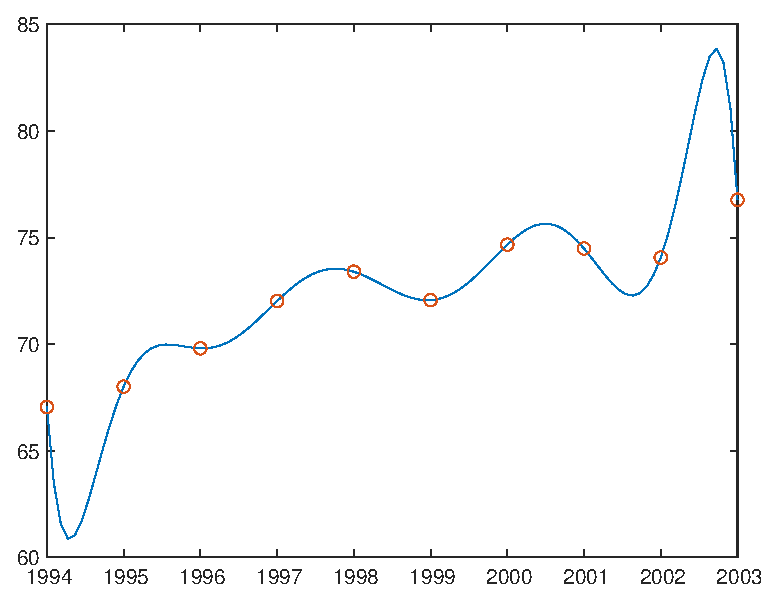
\includegraphics [width=4in]{main_04.eps}


\subsection*{PROBLEM 5-3 NUMERICAL INTEGRATION}

\begin{verbatim}
points_n_5_3={50,100,200,500,1000};
f_5_3=@(x)exp(3*x)*cos(x);

trape_5_3_res=cellfun(@nnl_mptrapeint,{[0,2*pi],[0,2*pi],[0,2*pi],...
    [0,2*pi],[0,2*pi]},points_n_5_3,{f_5_3,f_5_3,f_5_3,f_5_3,f_5_3});
simpson_5_3_res=cellfun(@nnl_mpsimpsonint,{[0,2*pi],[0,2*pi],[0,2*pi],...
    [0,2*pi],[0,2*pi]},points_n_5_3,{f_5_3,f_5_3,f_5_3,f_5_3,f_5_3});

syms x;
f_5_3_sym(x)=exp(3*x)*cos(x);
fi_5_3_sym(x)=int(f_5_3_sym);
exact_res_5_3=double(subs(fi_5_3_sym,x,2*pi)-subs(fi_5_3_sym,x,0));
clear x;

trape_5_3_e=trape_5_3_res-exact_res_5_3;
simpson_5_3_e=simpson_5_3_res-exact_res_5_3;

scatter(cell2mat(points_n_5_3),trape_5_3_e);
hold on
scatter(cell2mat(points_n_5_3),simpson_5_3_e);
\end{verbatim}

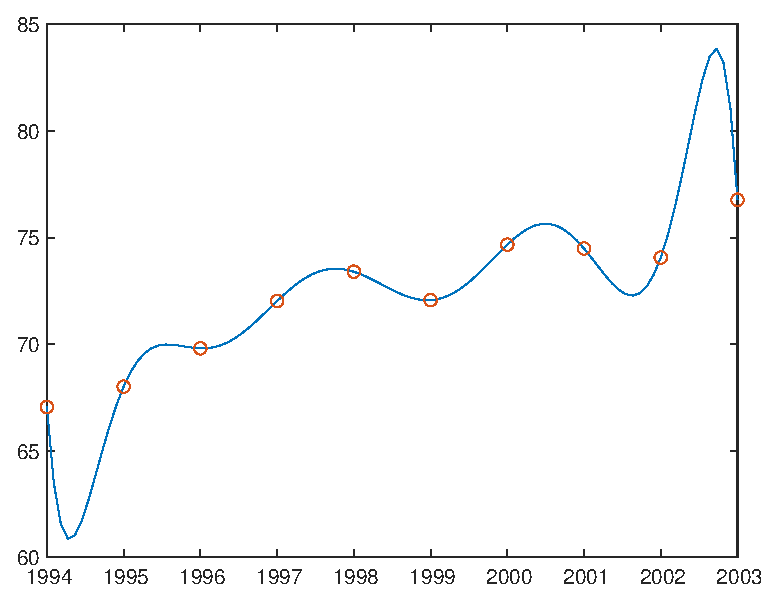
\includegraphics [width=4in]{main_05.eps}


\subsection*{PROBLEM 6-1 SOLAVE DIFFERETIAL EQUATION}

\begin{verbatim}
step_6_1={0.1,0.05,0.01};
f_6_1=@(t,u)2/t*u+t^2*exp(t);

rk_j=cellfun(@nnl_clsrk,{0,0,0},step_6_1,{[1,2],[1,2],[1,2]},...
    {f_6_1,f_6_1,f_6_1},'Uniformoutput',false);
clse_j=cellfun(@nnl_clseuler,{0,0,0},step_6_1,{[1,2],[1,2],[1,2]},...
    {f_6_1,f_6_1,f_6_1},'Uniformoutput',false);
adv_j=cellfun(@nnl_adveuler,{0,0,0},step_6_1,{[1,2],[1,2],[1,2]},...
    {f_6_1,f_6_1,f_6_1},'Uniformoutput',false);

for i=1:length(rk_j)
    plot(linspace(1,2,length(rk_j{i})),rk_j{i});
    hold on
end

for i=1:length(clse_j)
    plot(linspace(1,2,length(clse_j{i})),clse_j{i});
    hold on
end

for i=1:length(rk_j)
    plot(linspace(1,2,length(adv_j{i})),adv_j{i});
    hold on
end

syms x u(x);
f_6_1_sym=2/x*u+x^2*exp(x);
f_sym_6_1_sol=dsolve(diff(u)==2/x*u+x^2*exp(x),u(1)==0,x);
fplot(f_sym_6_1_sol,[1,2]);
clear x u;
legend;
\end{verbatim}

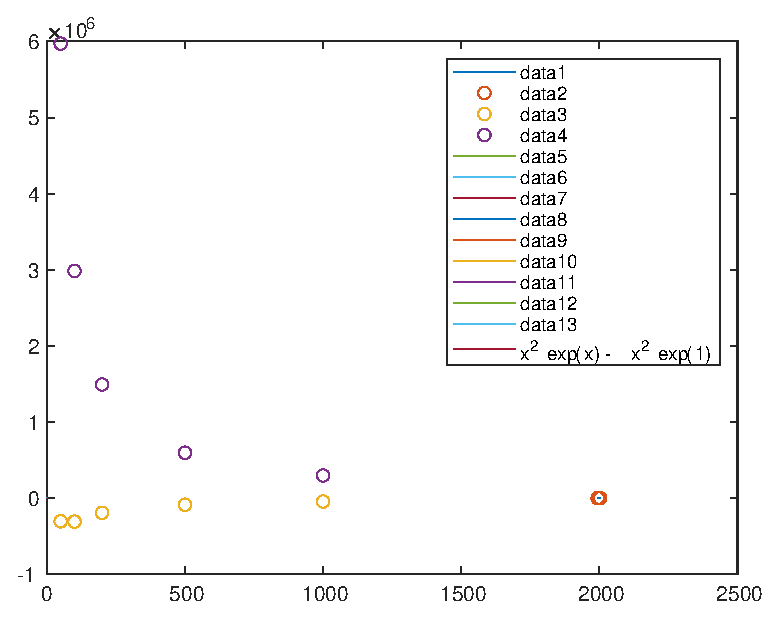
\includegraphics [width=4in]{main_06.eps}



\end{document}

